\section{Design Phase of the PlayStation Controller}
This is the design phase of PS controller.
\todo[inline]{write here}

%what is SEA
\subsection{Principle of Series Elastic Actuators (SEA)}
%TODO Alternatively, if the motors are non-backdriveable, a constant force can be created with only momentary motor voltage application.
The principle of series elastic actuators is relatively simple. The concept is explained in \cite{Pratt1995} which also mentions a more accurate and stable force control and the possibility of energy storage. An SEA is a normal actuation setup with an integrated elastic element. For this purpose a simple spring or a set of springs can be used. As it can be seen in figure \ref{fig:control_scheme} the control scheme is reduced to a simple distance-based control, while the output remains an equivalent force, given by Hooke's law.\\

\begin{figure}[h!]
	\centering
	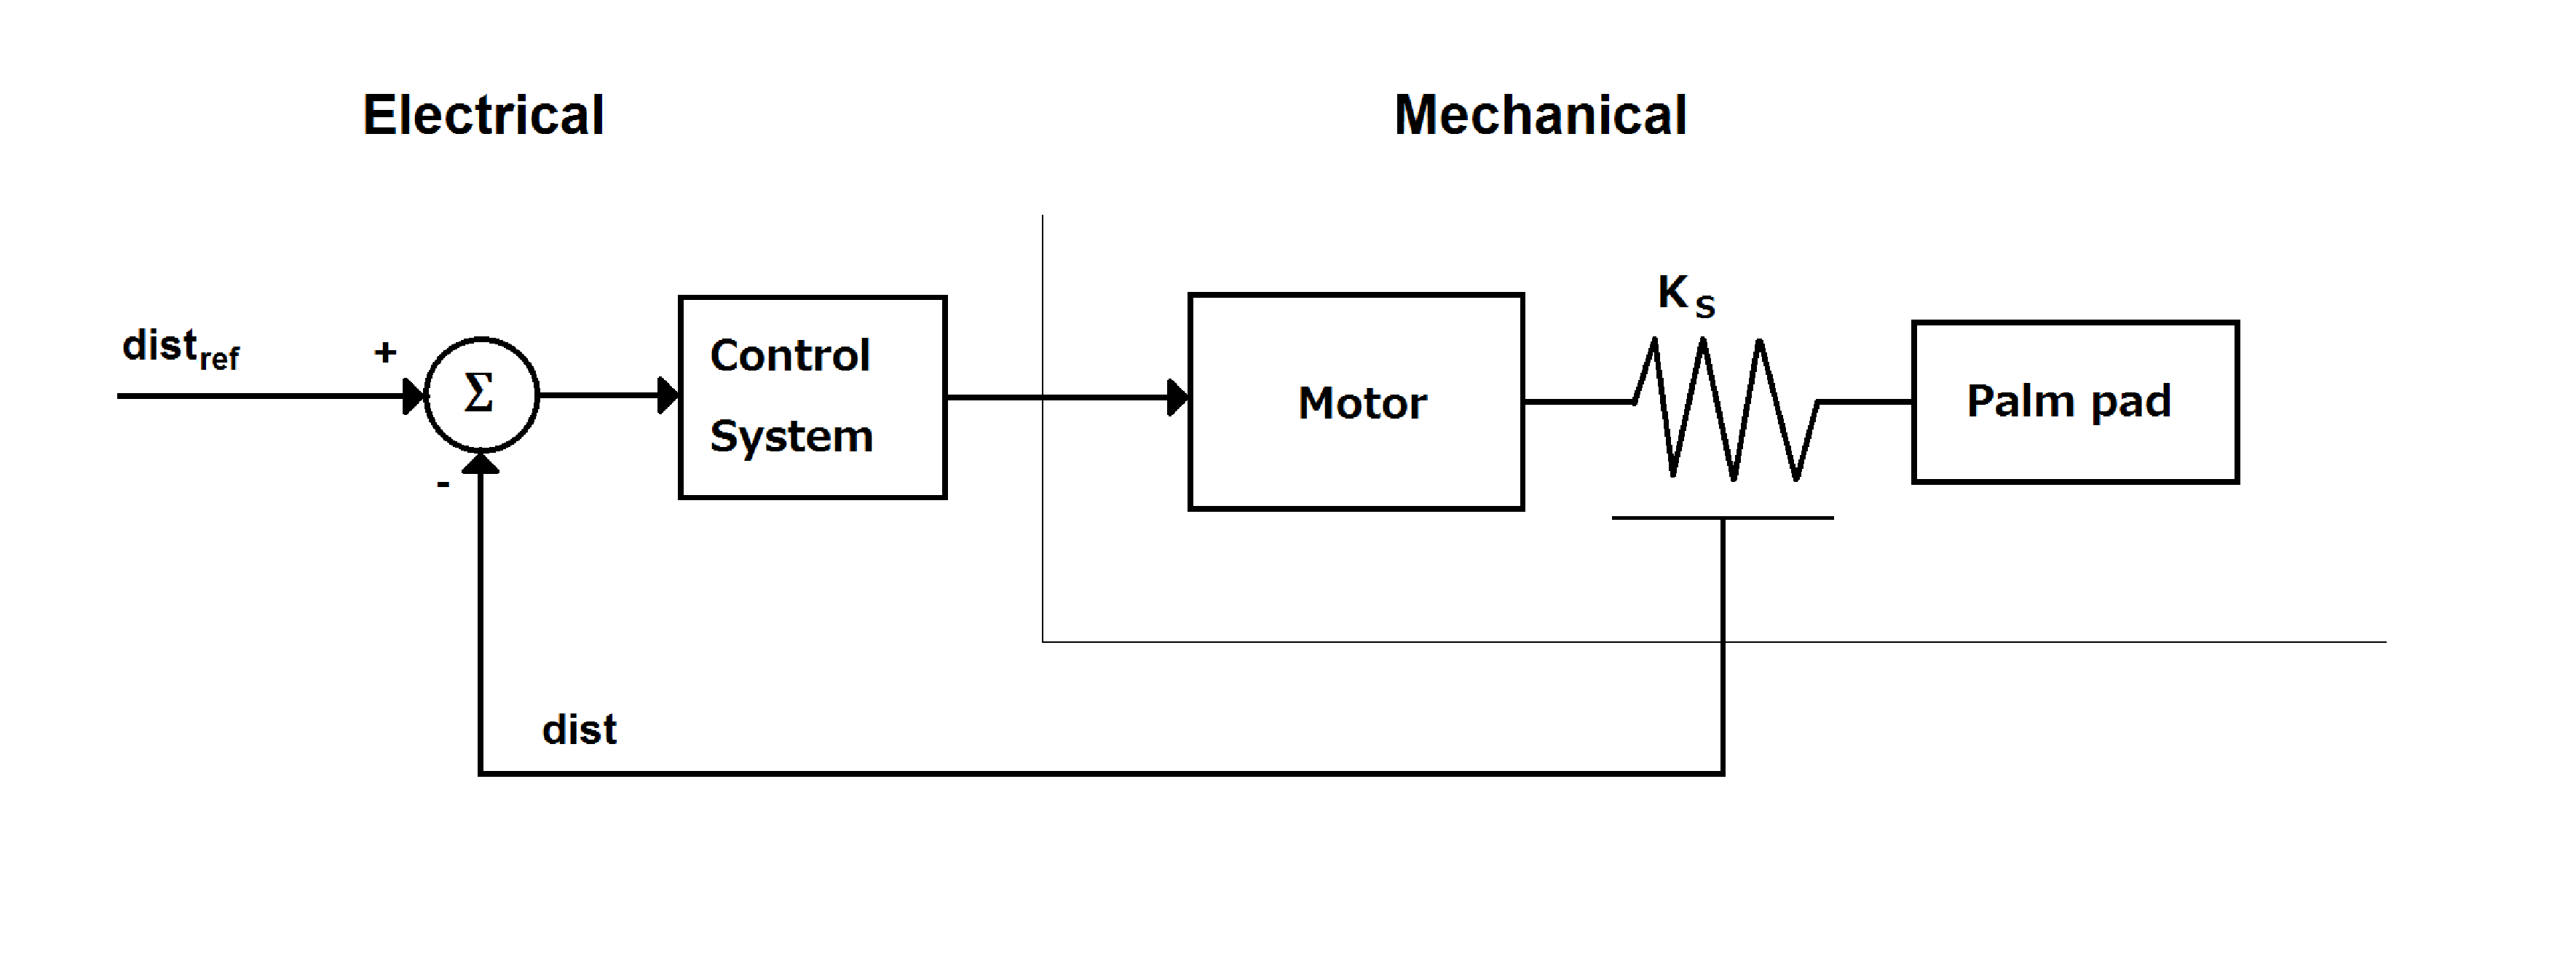
\includegraphics[width=0.7\linewidth]{Figs/control_scheme}
	\caption{Control scheme for the haptic feedback system.}
	\label{fig:control_scheme}
\end{figure}

An additional advantage is, that the elastic element is shock absorbent and stable for different environments. This means that the controller can be stable even when used with different grip stiffnesses.

A thorough study of an SEA design and its analysis has been made in \cite{Junior2016}, stating that the most important parameter in the system is the spring constant. Therefore, springs with several different spring constants have been used for the analysis of this research project.\\

\subsection{Implementation}
At first, several different SEA implementations, ranging from a car-jack system, wedge, cam, toothed bar, linear actuator or pneumatic based systems have been studied and analyzed. However, the clamp link based linear guideway controller (see figure \ref{fig:actuation_schematic}) seemed to fit best into the PlayStation-like casing. Also, the calculated force of $14$N was promising. Due to singularities in the design, the movement of the clamp link was restricted to $90^\circ$ and it was furthermore calculated, that the maximum stroke could be achieved within $100$ms.

\begin{figure}[h!]
	\centering
	\includegraphics[width=0.5\linewidth]{Figs/actuation_schematic.jpg}
	\caption{Initial schematic of the actuation design.}
	\label{fig:actuation_schematic}
\end{figure}

\subsection{Inspiration of the Design}
It is not far-fetched to search for inspiration in the domain of entertainment, if a user-friendly handheld controller is needed. The probably most famous controller is the one designed by PlayStation \footnote{\url{https://www.playstation.com/en-us/}}
\todo[inline]{check if i can call my controller PS contr.}, which can be used for a variety of applications. Due to this flexibility and the simple but elegant design, this work has opted for a similar design and used the PlayStation controller, as well as the design of the previous research as models. From now on, this controller design is called PlayStation controller.


%what it looks like in the end
\subsection{Design and Prototyping}
The 3D design of the PS controller can be seen in figure \ref{fig:PS_controller_design}.

\begin{figure}
    \centering
    \begin{minipage}{0.425\textwidth}
	    \begin{figure}[H]
		\centering
		\includegraphics[width=1.0\linewidth]{Figs/centric_shaft_controller_smaller_top_view_dir.jpg}
		%\caption{3D model of the PlayStation controller.}
		\label{fig:PS_controller_smaller}
	\end{figure}
	\end{minipage}
	\begin{minipage}{0.45\textwidth}
	    \begin{figure}[H]
		\centering
		\includegraphics[width=1.0\linewidth]{Figs/PS_controller_smaller_open_rend.jpg}
		%\caption{3D rendering of the PlayStation controller.}
		\label{fig:PS_controller_smaller_open_rend}
	    \end{figure}
	\end{minipage}
    
    \caption{3D model and rendering of the PlayStation controller.}
    \label{fig:PS_controller_design}
\end{figure}


This design of the controller aims at having a natural position for the hands, such that the user can hold the controller for a long time without having the hands in an awkward position. As it can be seen in the figure, the palm pads that transmit the feedback pressure to the palms are not directed perpendicularly towards the user, but rather outwards at a certain angle (refer to figure \ref{fig:PS_controller_design}). This can be seen as a drawback, since the user is expected to have the most intuitive feeling with a feedback opposing the driving direction (ie. perpendicular).

	
	
The dimensions of the controller are 220mm in length, 110mm in width and 70mm in height. The controller is unusually thick due to the feedback actuation design. This actuation design can be seen in figure \ref{fig:actuation_system_explained}. The motor shaft is rotating a clamp link which is attached to a 3D-printed part, called connecting link. This 3D-printed part is attached to the carriage, an also 3D-printed part called L-plate, and is screwed to the linear guideway. The L-plate is connected via a set of springs (different spring constants have been tested) to the palm pad, thus making it an SEA. The linear guideway keeps the palm pad in a linear motion.

\begin{minipage}{0.7\textwidth}
\begin{figure}[H]
	\centering
	\includegraphics[width=1.0\linewidth]{Figs/actuation_system_explained}
	\caption{Actuation system with legend.}
	\label{fig:actuation_system_explained}
\end{figure}
\end{minipage}
\begin{minipage}{0.29\textwidth}
	\begin{itemize}
    	\item (1) : Palm pad
    	\item (2) : Photoreceptor
    	\item (3) : L-plate
    	\item (4) : Connecting link
    	\item (5) : Clamp link
    	\item (6) : Motors
    	\item (7) : Linear guideway
    	\item (8) : Springs
    \end{itemize}
\end{minipage}

\subsection{Electrical Components}
To have a functional controller, several requirements had to be met. First of all, an actuation system was necessary to provide the feedback. In addition to that, the user shall be able to navigate the robot, which has been realized with potentiometer based joysticks. To close the loop and create the desired force output, it was furthermore necessary to measure the compression of the springs. This has been realized with a simple photoreceptor as a distance sensor.

\subsubsection{Motors}
The motors play an important role on the output force of the controller, as well as the achievable control speed. There were motors with two different reduction gear ratios available in the laboratory. They stem from Faulhaber's series called \textbf{2619 024 SR IE2-16} and their reduction ratios were \textit{33:1} and \textit{112:1}. The maximum intermittent output torques are $100$mNm and $180$mNm respectively. However, due to the reduction stages, the efficiency is around $60\%$. The maximally applicable voltage is of $24$V, for motor protection however, the motor voltage has been limited to $20$V during normal operation.

\subsubsection{Joysticks}
The joysticks are conventional 2-axes potentionmeters. The series number is \textbf{P-04048} and they have been bought at Akizukidenshi store.

\subsubsection{Photoreceptors}
The photoreceptors are the \textbf{TPR-105} from \textit{GENIXTEK CORP}. The circuit can be seen in figure \ref{fig:tpr105_circuit}. The components chosen are $R_1 = 330\Omega$ and $R_2 = 27k\Omega$.
	
\begin{figure}[h!]
	\centering
	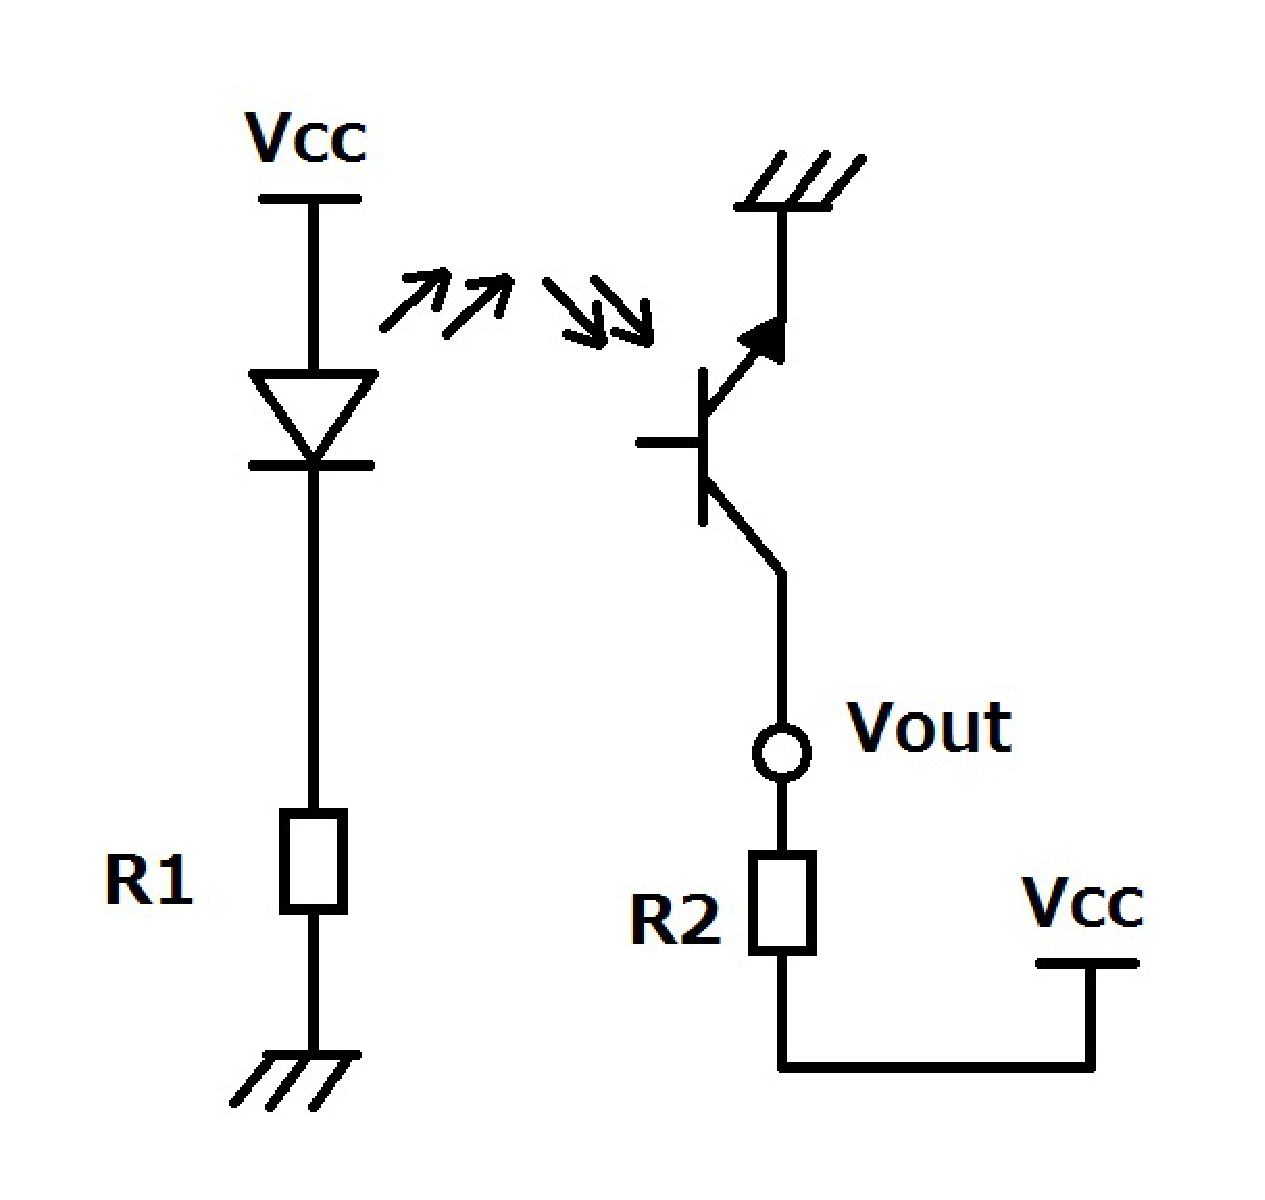
\includegraphics[width=0.2\linewidth]{Figs/tpr105_circuit}
	\caption{Photoreceptor circuit.}
	\label{fig:tpr105_circuit}
\end{figure}
The photoreceptors' working principle is based on detecting the amount of reflected light. This controls the base current $i_B$ of the transistor in the schematic. This base current then determines the collector current $i_C$. Specific to this setup, the distance and therefore the output force controls the amount of light that is reflected on the wall of the palm pad. Therefore, we have:

\begin{equation}
F_{output} = k_{eq} \Delta x \propto i_B
\end{equation}
\begin{equation}
i_C = h_{FE} i_B
\end{equation}
\begin{equation}
V_{out} = V_{CC} - h_{FE} R_2 i_B = V_{CC} - K R_2 \Delta x
\end{equation}

Where $h_{FE}$ is the forward current gain and $K$ is a constant given by $h_{FE} k_{eq}$.
	
The two resistor values have been empirically found to have the highest sensitivity but not saturating the measurement. The sensitivity decreases with a smaller resistor, since at a certain point, the Arduino cannot detect a change in voltage anymore. Saturation occurs, when the value of $R_2$ is too high. Also, it has been opted for keeping the operational distance in the linear range of the sensing position characteristic (see datasheet).\todo[inline]{reference datasheet in appendices or references?}


\paragraph{Identification of Operational Range (Photoreceptor)}
To find the receptor values at maximum compression of the springs, a simple test has been made, where one time $0$V has been applied to the motors, and another time $20$V has been applied. The results can be seen in figure \ref{fig:max_volt_applied_plot}.
	
\begin{figure}[h!]
	\centering
	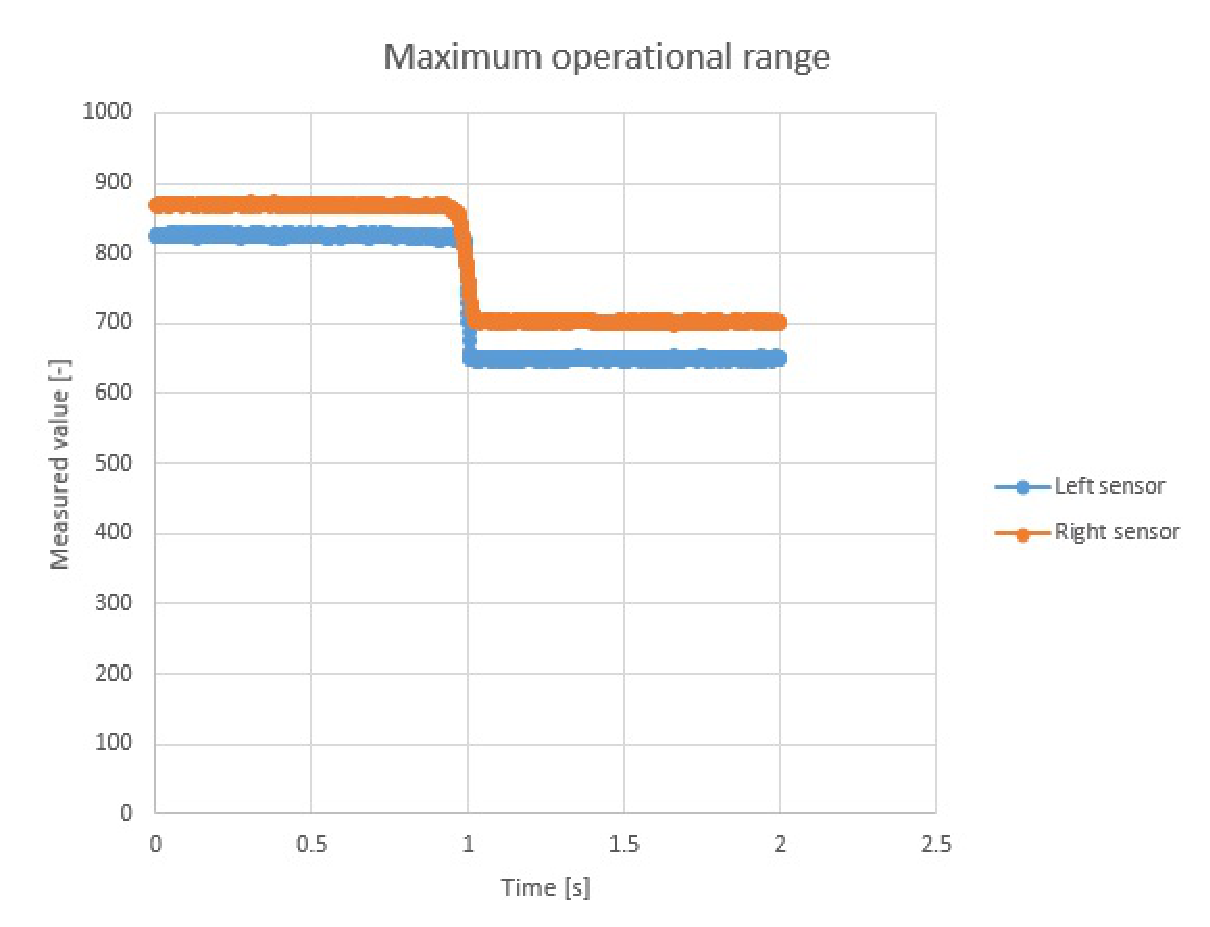
\includegraphics[width=0.6\linewidth]{Figs/max_volt_applied_plot}
	\caption{Operational range of photoreceptor with springs at rest and in full compression.}
	\label{fig:max_volt_applied_plot}
\end{figure}
	
The values that have been found to be the limiting values are resumed in table \ref{tab:oper_range_PS}.

\todo[inline]{Update these values in table}
\begin{figure}[h!]
	\centering
	\begin{tabular}{|l|c|c|c|c|c|}
    	\hline
		& Sensor reading & Distance & Sensor reading & Distance & Max output  \\
		& MAX (rest) & (rest) & MIN (compression) & (compression) & force \\ \hline \hline
		Left side & 830 & 2.35mm & 650 & 4mm & 9.9N \\ \hline
		Right side & 870 &2.2mm & 700 & 4mm & 10.8N \\ \hline
	\end{tabular}
	\caption{Identified operational range for the photoreceptors in the PlayStation controller.}
	\label{tab:oper_range_PS}
\end{figure}
	
Using these values, the photoreceptor measurements can be mapped to this range with an 8-bit value. This means that $0$ is no compression and $255$ is fully achievable compression. In the Arduino software these values have been slightly adapted (see table \ref{tab:programming_params}), to ensure a natural feeling, even when the sensor has some peak values. 


\subsection{Mechanical Components}
From the mechanical point of view, the spring implementation is the most essential part. However, there are other components that have an impact on the output force, the clamp link for instance, whose length acts as a lever. Other minor but non-negligible components are the linear guideway and the coupling.

\subsubsection{Springs}
\todo[inline]{write about importance of length, compressibility, stiffness, arrangement}
The springs are the most crucial part of the whole system. Not only is the output force determined by the spring constant and the compression rate, but also the length and arrangement of the springs have a major impact on the feeling of the controller. Intensive testing has shown that the arrangement has to be symmetric with preferably uniform springs. If springs with two different spring coefficients are used at the same time, the compression becomes rapidly asymmetric and the feedback feels unnatural. Also, if the springs are too long, then

For the final controller design, a total of four springs (\textbf{WT4-5}), arranged symmetrically on the palm pad have been used. The springs have a spring constant of $k_s = 1.5$N/mm which corresponds to an equivalent spring constant of $k_{eq} = 6$N/mm. They are distributed around the palm pad, where in their middle a distance sensor (called photoreceptor) has been attached, to measure the distance between the L-plate (carriage) and the palm pad. It therefore measures the compression of the springs, which can be related to the output force by Hooke's law as:
\begin{equation}
	F = k_{eq}x 	
\end{equation}

The setup of the carriage with the springs and the palm pads can be seen in figure \ref{fig:setup_annotated}.
\begin{figure}[h!]
	\centering
	\includegraphics[width=0.4\linewidth]{Figs/setup_annotated}
	\caption{Schematic of the spring system setup.}
	\label{fig:setup_annotated}
\end{figure}

\subsubsection{Linear Guideway}
The linear guideway is the model \textbf{LS-827} from \textit{THK}. Its maximum stroke is $13$mm, which is enough for compression the springs, as well as indenting the operators palms to a certain extent. This guideway restricts the movement of the carriage to a unidirectional one.

\subsubsection{Coupling}
The coupling (\textbf{SCPS16-3-5}) and its functionality are straightforward.

\subsubsection{Clamp Link}
The clamp link acts as a lever pushing the carriage in its guideway. Different lengths have been tested, but the model in the final design is \textbf{CLKWS5-3-20}. It converts the rotational motion of the motor shaft to an almost linear motion on the other end. To compensate for the parasitic motions, an additional element called connecting link (see figure \ref{fig:actuation_system_explained}) has been designed.  



\newpage